% !TEX root = ../../main.tex
\section{Watershed Methods}\label{sec:rw_watershed_methods}

The idea of watersheds has been introduced by \citet{beucher_1979_workshop}.

Other watersheds \citep{vinent_1991_pami,najman_1994_sp,roerdink_2000_finf,bertrand_2005_jmiv,cousty_2009_pami}.


The watershed algorithm can be often described with the following analogy:

\paragraph{Water Flooding:} A grayscale  image can be interpreted as hight map (see \cref{fig:ws_2d_map}, \cref{fig:ws_2d_map3d}).
The water level is raised as shown in \cref{fig:ws_a} - \cref{fig:ws_f}.
A watershed is wherever the water of two adjacent valleys is meeting (see \cref{fig:ws_e},\cref{fig:ws_f} and \cref{fig:ws_2d_lines}).


% watersheds illustrated
\begin{figure}
    \centering
    \subfloat[1d Image Data]{ \label{fig:ws_a}
        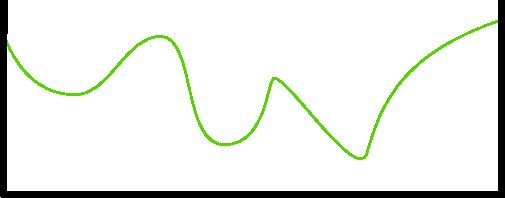
\includegraphics[width=0.25\textwidth]{fig/ws_no_no.pdf}
    }
    \hspace{0.5cm}
    \subfloat[Local minima]{  \label{fig:ws_b}
        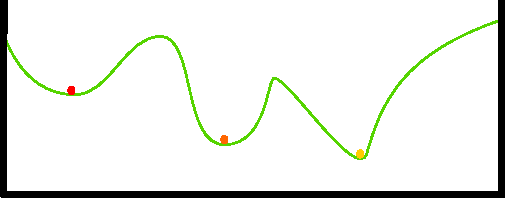
\includegraphics[width=0.25\textwidth]{fig/ws_no.pdf}
    }
    \hspace{0.5cm}
    \subfloat[flooding starts]{  \label{fig:ws_c}
        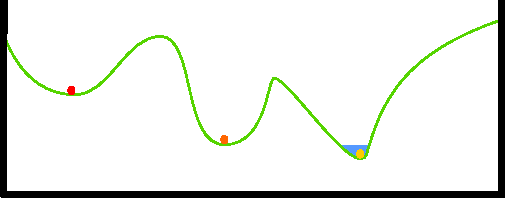
\includegraphics[width=0.25\textwidth]{fig/ws3.pdf}
    }
    \\
    \subfloat[flooding]{  \label{fig:ws_d}
        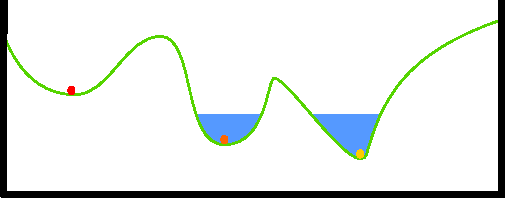
\includegraphics[width=0.25\textwidth]{fig/ws2.pdf}
    }
    \hspace{0.5cm}
    \subfloat[watershed 1]{  \label{fig:ws_e}
        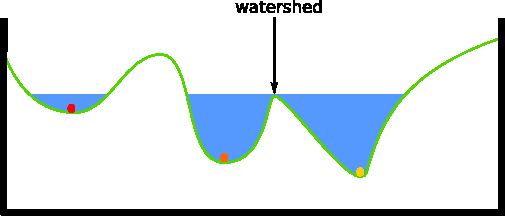
\includegraphics[width=0.25\textwidth]{fig/ws1.pdf}
    }
    \hspace{0.5cm}
    \subfloat[watershed 2]{ \label{fig:ws_f}
        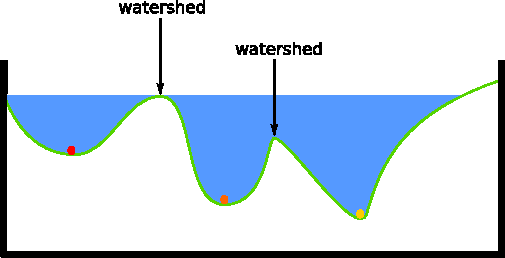
\includegraphics[width=0.25\textwidth]{fig/ws0.pdf}
    }
    \\ % 2D Watersheds
    \subfloat[$ $]{ \label{fig:ws_2d_map}
        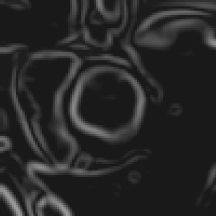
\includegraphics[height=0.26\textwidth]{fig/ws2d0.png}
    }
    \hspace{0.1cm}
    \subfloat[$ $]{ \label{fig:ws_2d_map3d}
        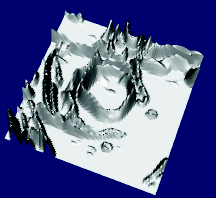
\includegraphics[height=0.26\textwidth]{fig/ws2d1.png} 
    }
    \hspace{0.1cm}
    \subfloat[$ $]{ \label{fig:ws_2d_lines}
        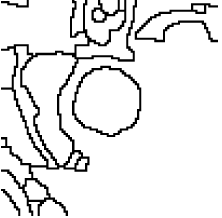
\includegraphics[height=0.26\textwidth]{fig/ws2d2.png}
    }

    \addtocontents{lof}{%
        \vspace{1cm}
        \protect\centerline{%
            \protect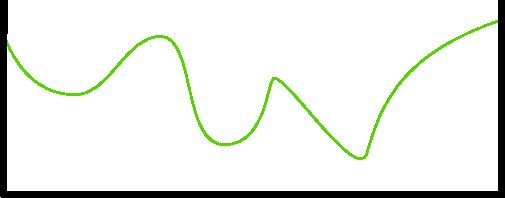
\includegraphics[width=.075\linewidth]{fig/ws_no_no.pdf}  \hspace{0.2cm}
            \protect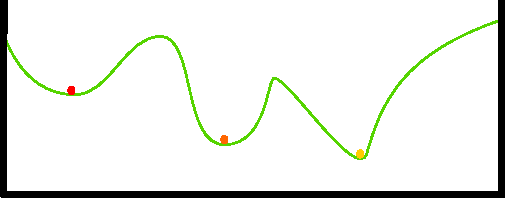
\includegraphics[width=.075\linewidth]{fig/ws_no.pdf}\hspace{0.2cm}
            \protect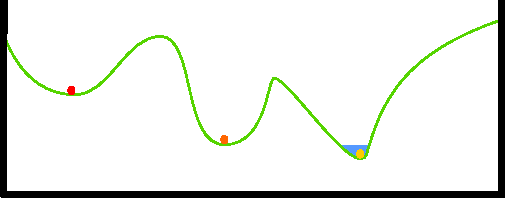
\includegraphics[width=.075\linewidth]{fig/ws3.pdf} 
        }%
        \vspace{0.2cm}
        \protect\centerline{%
            \protect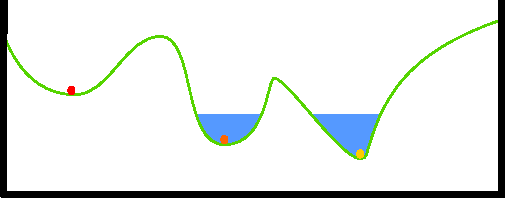
\includegraphics[width=.075\linewidth]{fig/ws2.pdf}  \hspace{0.2cm}
            \protect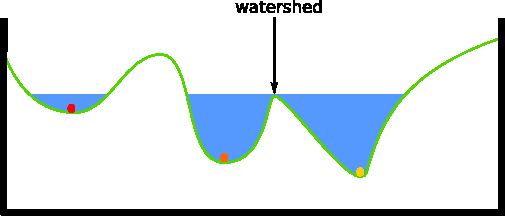
\includegraphics[width=.075\linewidth]{fig/ws1.pdf} \hspace{0.2cm}
            \protect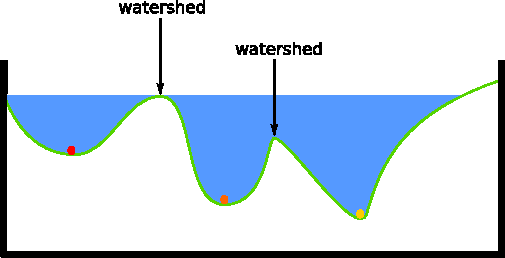
\includegraphics[width=.075\linewidth]{fig/ws0.pdf}%
        }%
        \vspace{0.2cm}
        \protect\centerline{%
            \protect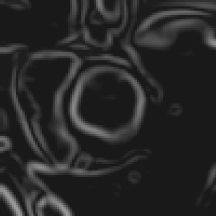
\includegraphics[height=.075\linewidth]{fig/ws2d0.png}  \hspace{0.2cm}
            \protect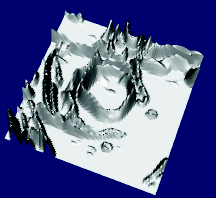
\includegraphics[height=.075\linewidth]{fig/ws2d1.png} \hspace{0.2cm}
            \protect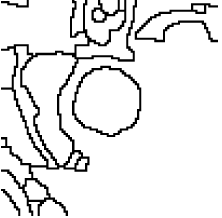
\includegraphics[height=.075\linewidth]{fig/ws2d2.png}%
        }%
    }%
    \caption[Illustration of watershed flooding process]{ 
        Illustration of watershed flooding process.
        The water level raises, and the watersheds are at the positions where water from different catchment basins is meeting.
    } \label{fig:watersheds_1d}
\end{figure}





\citet{couprie_2011_pami} proposed an algorithm, \emph{power-watershed}, a generalization of \citep{RANDOM_WALKER, GRAPH_CUT,WATHERSHEDS,sinop_2007_iccv}.
They define the following model.
\begin{align}\label{eq:power_watershed}
\min_x \sum_{e_{ij} \in E}  w_{ip}^p |x_i-x_j|^q + \sum_{v_i } w_{Fi}^p |x_i|^q + \sum_{v_i } w_{Bi}^p |x_i-1|^q \\
s.t. \hspace{0.35cm} x(F)=1, \hspace{0.5cm} x(B)=0
\end{align}
Setting $p$ to 1 will lead to the methods proposed by \citet{sinop_2007_iccv}.
\Citet{allene_icv_2010} pointed out when $p=1$ and $q \rightarrow \infty$, solving
\cref{eq:power_watershed} is equivalent to applying a minimum spanning forest algorithm.




\citet{straehle_2011_miccai} proposed a watershed based method for interactive segmentation
of neural volume electron  microskopy images.
They show how a background prior be be efficiently integrated into watersheds,
and that this prior is beneficial for neuro data.
In addition \citet{straehle_2012_cvpr} proposed an uncertainty estimator for
guided interactive segmentation based on watersheds.
